%%%%%%%%%%%%%%%%%%%%%%%%%%%
% Motivation and construction of the FRT Index
% Christopher Gandrud
% 21 March 2014
%%%%%%%%%%%%%%%%%%%%%%%%%%%%

\documentclass[a4paper]{article}
\usepackage{fullpage}
\usepackage[authoryear]{natbib}
\usepackage{setspace}
    \doublespacing
\usepackage{hyperref}
\hypersetup{
    colorlinks,
    citecolor=black,
    filecolor=black,
    linkcolor=cyan,
    urlcolor=cyan
}
\usepackage{amsmath}
\usepackage{dcolumn}
\usepackage{booktabs}
\usepackage{url}
\usepackage{tikz}
\usepackage{todonotes}
\usepackage[utf8]{inputenc} 
\usepackage{graphicx}
\usepackage{longtable}
\usepackage{todonotes}

%%%%%%%%% Title
\title{Measuring Financial Regulatory Transparency}

\author{Mark Copelovich \\ \emph{University of Wisconsin, Madison} \\[0.5cm] Christopher Gandrud and Mark Hallerberg \\ 
    {\emph{Hertie School of Governance}}\footnote{Friedrichstra{\ss}e 180. 10117 Berlin, Germany. Contact email: \href{mailto:gandrud@hertie-school.org}{gandrud@hertie-school.org}. All material for replicating the FRT Index and the analysis in this paper can be found at: \url{https://github.com/FGCH/FRTIndex}.}}


\begin{document}

\maketitle

%%%%%%%%% Abstract
\begin{abstract}
\noindent \emph{Early working draft. Comments welcome.} \\
For financial supervision to be effective, regulators need have accurate information about financial sector activities. For the public to be able to hold supervisors accountable they need access to the information financial supervisors have about the health of the banking system. In this paper we use Bayesian item response theory to create a new global and comparable Financial Regulatory Transparency (FRT) Index. The Index currently covers the years 1998 through 2011. It captures high income countries', those most likely to have developed financial systems, reporting to the World Bank's Global Financial Development data set. The Index is a distinct indicator of governments' willingness to gather and make information about their financial systems and regulators' actions publicly available. 
\end{abstract}

In previous research we have found that even within the relatively homogeneous European Union with supranational authorities tasked with gathering and reporting aggregate financial data from member states there is considerable variation in what is actually reported \cite[see][]{Gandrud2014a}. We currently lack a comparable cross-national way of measuring country's level of financial regulatory transparency. In this paper we use a Bayesian Item Response Theory (IRT) approach

\section{Creating the FRT Index}

We treat financial regulatory transparency as an unobserved latent variable that effectively summarizes countries likelihood of reporting yearly data that is included in the World Bank's Global Financial Development data (GFDD) set first created by \cite{Cihak2012}.\footnote{Access to the most updated version of the data set is available through \url{http://data.worldbank.org/data-catalog/global-financial-development} Accessed February 2014.}

\subsection{Included indicators}

To measure financial supervisory transparency we first gathered data on whether or not governments reported data on a subset of indicators that are included in the World Bank's Global Financial Development data set. We followed Hollyer et al.`s \citeyearpar{Hollyer2014} criteria for inclusion of variables and countries. First, we only include indicators that are reported by at least one country for each year in the period 1998-2011. This gave us the greatest coverage of indicators that are comparable across countries. Second, we excluded all indicators that were explicitly gathered for only a subset of countries. As such we avoided including data where the primary source was the Bank for International Settlements. Third, we did not include any indicator that was primarily from a non-governmental source. This included both indicators from World Bank Sponsored surveys, such as the Global Financial Inclusion Survey and the Enterprise Survey. It also included data primarily derived from sources such as Swiss Re's Sigma Reports, Standard \& Poor, Bankscope, and Bloomberg. Fourth, we did not include variables that are linear combinations of other variables. Fifth, we did not include variables that were simply references to the same quantity in different units. Sixth, we aim to focus on countries that have relatively highly developed banking systems. As such we include only countries and jurisdictions that the World Bank classifies as 'high income'.\footnote{We include both OECD and non-OECD high income countries.} Countries with levels of income this low likely do not have financial systems sophisticated enough to have the quantities reported in the indicators. 

Using these criteria our model has 60 countries, 21 items, and 12 years (1998-2011). Table~\ref{IndTable} shows the list of indicator items and descriptions.  

\begin{table}[ht]
    \caption{Indicators included in the FRT Index from the World Bank's Global Financial Development data set}
    \label{IndTable}
    \vspace{0.3cm}
    \scalebox{0.95}{
        % latex table generated in R 3.0.2 by xtable 1.7-1 package
% Thu Feb 20 10:58:09 2014
{\scriptsize
\begin{tabular}{llll}
  \hline
SeriesCode & Indicator.Name & Source & Periodicity \\ 
  \hline
GFDD.DI.01 & Private credit by deposit money banks to GDP (\%) & IFS/IMF & 1961-2011 \\ 
  GFDD.DI.02 & Deposit money banks' assets to GDP (\%) & IFS/IMF & 1961-2011 \\ 
  GFDD.DI.03 & Nonbank financial institutions’ assets to GDP (\%) & IFS/IMF & 1961-2011 \\ 
  GFDD.DI.04 & Deposit money bank assets to deposit money bank assets and central bank assets (\%) & IFS/IMF & 1960-2011 \\ 
  GFDD.DI.05 & Liquid liabilities to GDP (\%) & IFS/IMF & 1961-2011 \\ 
  GFDD.DI.06 & Central bank assets to GDP (\%) & IFS/IMF & 1961-2011 \\ 
  GFDD.DI.07 & Mutual fund assets to GDP (\%) & World Bank & 1980-2011 \\ 
  GFDD.DI.08 & Financial system deposits to GDP (\%) & IFS/IMF & 1961-2011 \\ 
  GFDD.DI.11 & Insurance company assets to GDP (\%) & World Bank & 1980-2011 \\ 
  GFDD.DI.12 & Private credit by deposit money banks and other financial institutions to GDP (\%) & IFS/IMF & 1961-2011 \\ 
  GFDD.DI.13 & Pension fund assets to GDP (\%) & World Bank & 1990-2011 \\ 
  GFDD.DI.14 & Domestic credit to private sector (\% of GDP) & World Bank & Annual: \\ 
  GFDD.EI.02 & Bank lending-deposit spread & IFS/IMF & 1980-2011 \\ 
  GFDD.EI.08 & Credit to government and state owned enterprises to GDP (\%) & IFS/IMF & 1980-2011 \\ 
  GFDD.OI.02 & Bank deposits to GDP (\%) & IFS/IMF & 1961-2011 \\ 
  GFDD.OI.07 & Liquid liabilities in millions USD (2000 constant) & IFS/IMF & 1960-2011 \\ 
  GFDD.OI.13 & Remittance inflows to GDP (\%) & World Bank & 1970-2011 \\ 
  GFDD.SI.02 & Bank nonperforming loans to gross loans (\%) & IFSI/IMF & 1998-2011 \\ 
  GFDD.SI.03 & Bank capital to total assets (\%) & IFSI/IMF & 1998-2011 \\ 
  GFDD.SI.04 & Bank credit to bank deposits (\%) & IFS/IMF & 1960-2011 \\ 
  GFDD.SI.05 & Bank regulatory capital to risk-weighted assets (\%) & IFSI/IMF & 1998-2011 \\ 
  GFDD.SI.07 & Provisions to nonperforming loans (\%) & IFSI/IMF & 1998-2011 \\ 
   \hline
\end{tabular}
}

    }
    {\scriptsize{Sources Key:\\ 
    IFS = International Financial Statistics\\
    IMF = International Monetary Fund}}
\end{table}

\subsection{The model}

As in \cite{Hollyer2014} we let $y_{j,c,t} \in \{0,\; 1\}$ indicate a variable that is 1 when a country $c$ reports a GFDD variable $j$ in year$t$. It is 0 otherwise. We then estimate the model:

\begin{equation}
    \mathrm{Pr}(y_{j,c,t} = 1|transparency_{c,t} = \mathrm{logit}(\delta_{j} + \beta_{j}transparency_{c,t})
\end{equation}

The following parameters are estimated in the model:

\begin{itemize}
    \item $\delta_{j}$ is the difficulty parameter of item $j$,
    \item $\beta_{j}$ the discrimination parameter for item $j$,
    \item $transparency_{c,t}$ is the estimated propensity of a given country-year $c,t$ to disclose financial regulatory data
\end{itemize}

\noindent $\delta_{j}$ indicates on average the degree to which countries report indicator $j$ in the GFDD over the entire time span. $\beta_{j}$ indicates how well reporting item $j$ predicts reporting other items. 

As \cite{Hollyer2014} note, simply taking the fraction of items a country reports in a given year as an indicator of transparency would be equivalent to assuming that $\delta_{j}$ and $\beta_{j}$ are constant across all variables. However, some items are 'harder' to report than others as they reveal information that regulators may find to be more sensitive for whatever reason. The IRT approach here allows us to not have to make this assumption. Instead we directly estimate the degree to which countries find it `difficult' to report items and how reporting an item (or not) is related to non-reporting of other items.

In order to fix the scale and location of the the FRT Index we followed \cite{Hollyer2014} by subtracting it by the mean and dividing by the standard deviation of the first year of the data set (1998) at each iteration. 

The Index values in 1998 are draw from a diffuse normal prior ($Transparency_{c,1980} \sim N(0,\:100)$) before recentering. For each transparency value after 1998 we used a system of random-walk priors such that $transparency_{c,t} \sim N(transparency_{c,t-1,\frac{1}{\tau_{c}}}) \forall t > 1$, where $\tau_{c}$ acts as a country-specific smoothing parameter. Each $\tau_{c}$ is estimated with the prior $\tau_{c} \sim Gamma(20,\:0.25)$ \citep[for more details see][8]{Jackman2009,Hollyer2014}. Finally, we used diffuse priors when estimating the discrimination and difficulty parameters:

\begin{equation}
    \begin{pmatrix}
      \delta{j} \\
      \beta_{j}
    \end{pmatrix} 
    \sim N 
    \left(
        \begin{pmatrix} 
            0 \\
            0 
        \end{pmatrix}
            ,\:
        \begin{pmatrix} 
            100 & 0 \\
            0 & 100
        \end{pmatrix}
    \right). 
\end{equation}

We estimated the model using a Markov Chain Monte Carlo algorithm using Jags 3.3.0 \citep{Plummer2003}.\footnote{The original Jags model can be found at: \url{https://raw.githubusercontent.com/FGCH/FRTIndex/master/source/BasicModel_V1.bug}. The R \citep{RCite} source code needed to download the underlying indicators and run the Jags model is available at: \url{https://raw.githubusercontent.com/FGCH/FRTIndex/master/source/FRTIndex_CreatorV2.R}. The later source code dynamically generates the Jags model.} We estimated two chains using 10,000 iterations each including burn-ins of 5,000 iterations. Please see the Supplementary Materials for convergence diagnostics.\todo{Need to do once the full model has been run.} 

\todo[inline]{Model fit discussion here}

\section{Description and Validity}


\subsection{The FRT Index}

Figures \ref{FRT_1998}, \ref{FRT_2007}, and \ref{FRT_2011} provide snapshots of the Financial Regulatory Transparency Index in the years 1998 (the Index's first year), 2007, and 2011 (the Index's current end year). Higher scores on the FRT Index indicate higher financial regulatory transparency.

We should first notice that the index passes a face validity test. There is a noticeable cluster of countries with very low FRT scores. These countries include the Bermuda, Cayman Islands, the Isle of Man, and Monaco. All of these jurisdictions are known for their banking secrecy, often as explicit policy decisions to attract capital from those seeking to avoid paying taxes in their home jurisdictions. At the high end of the scale we also see countries that have been known for their transparency. \cite{Gandrud2014a} noted a high level of financial regulatory transparency in the United States' financial regulatory reporting practices relative to practices among many European Union countries. As we would expect from this work, the United States is regularly placed among the countries with the highest FRT score.  

Changes in countries' FRT scores over time also reflect substantively meaningful policy changes. Hungary is a prime example, in 1998 it is estimated to have one of the highest FRT scores. \todo{Mark H. COULD YOU WRITE THIS UP?}

\begin{figure}
    \caption{Financial Regulatory Transparency Index in 1998}
    \label{FRT_1998}
    \begin{center}
        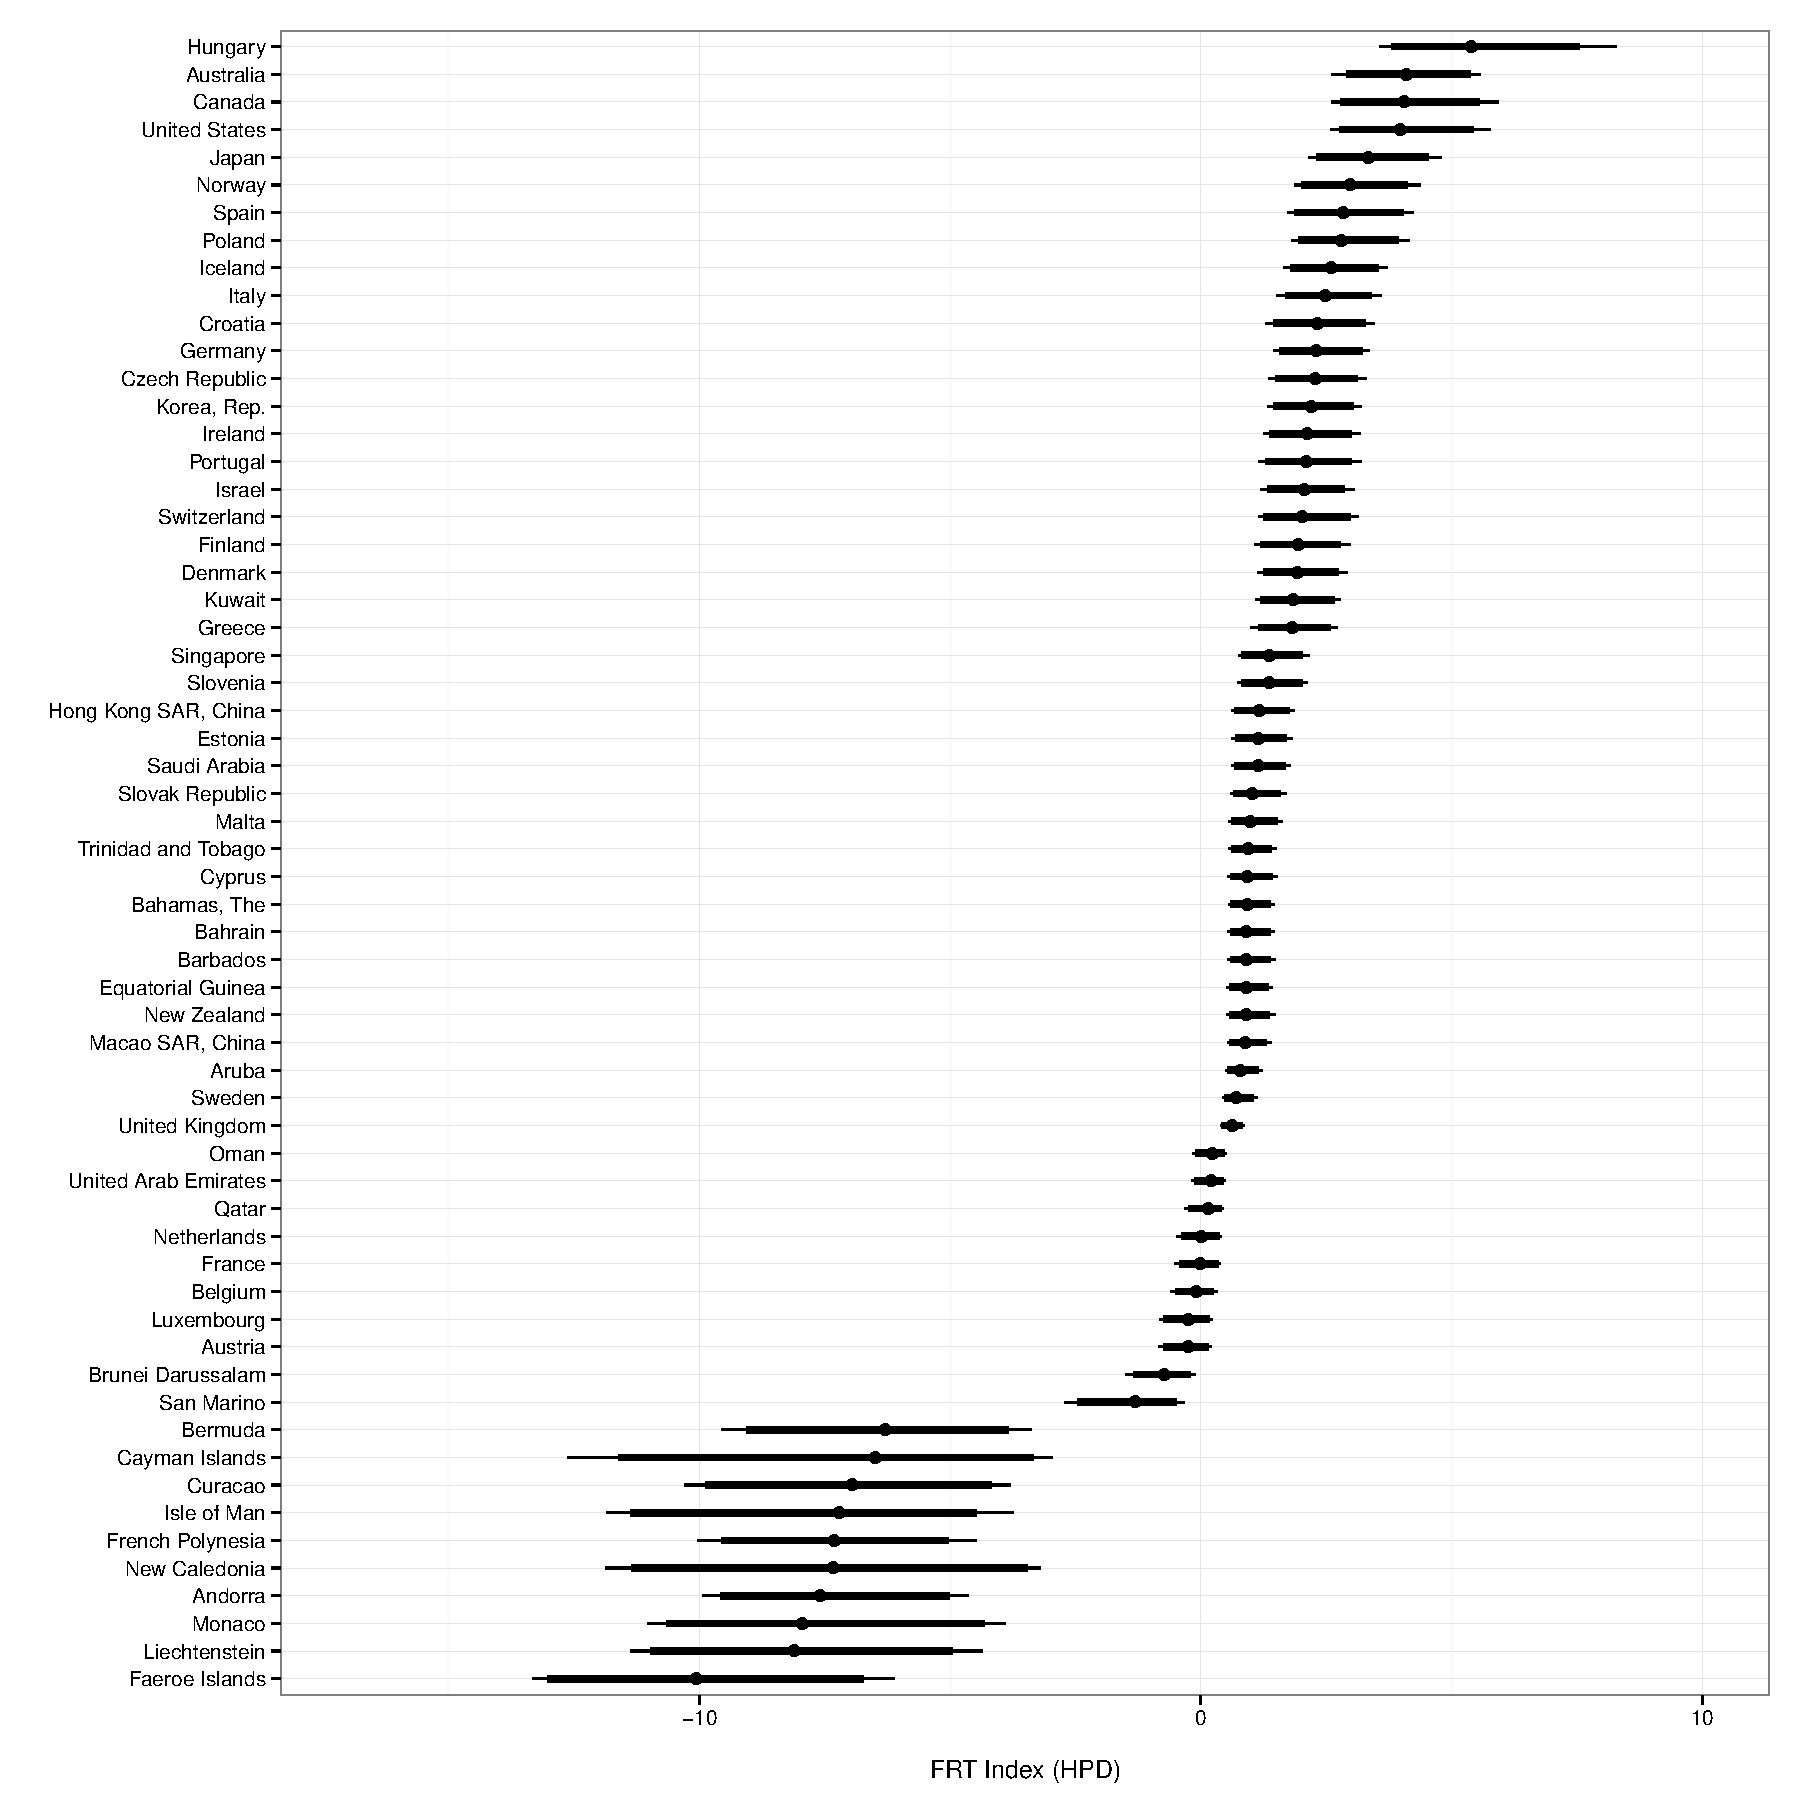
\includegraphics[scale=0.45]{figures/FRT_1998}
    \end{center}
    {\scriptsize{Thin lines represent the 95\% highest posterior density interval. Thick lines represent the 90\%.}}
\end{figure}

\begin{figure}
    \caption{Financial Regulatory Transparency Index in 2007}
    \label{FRT_2007}
    \begin{center}
        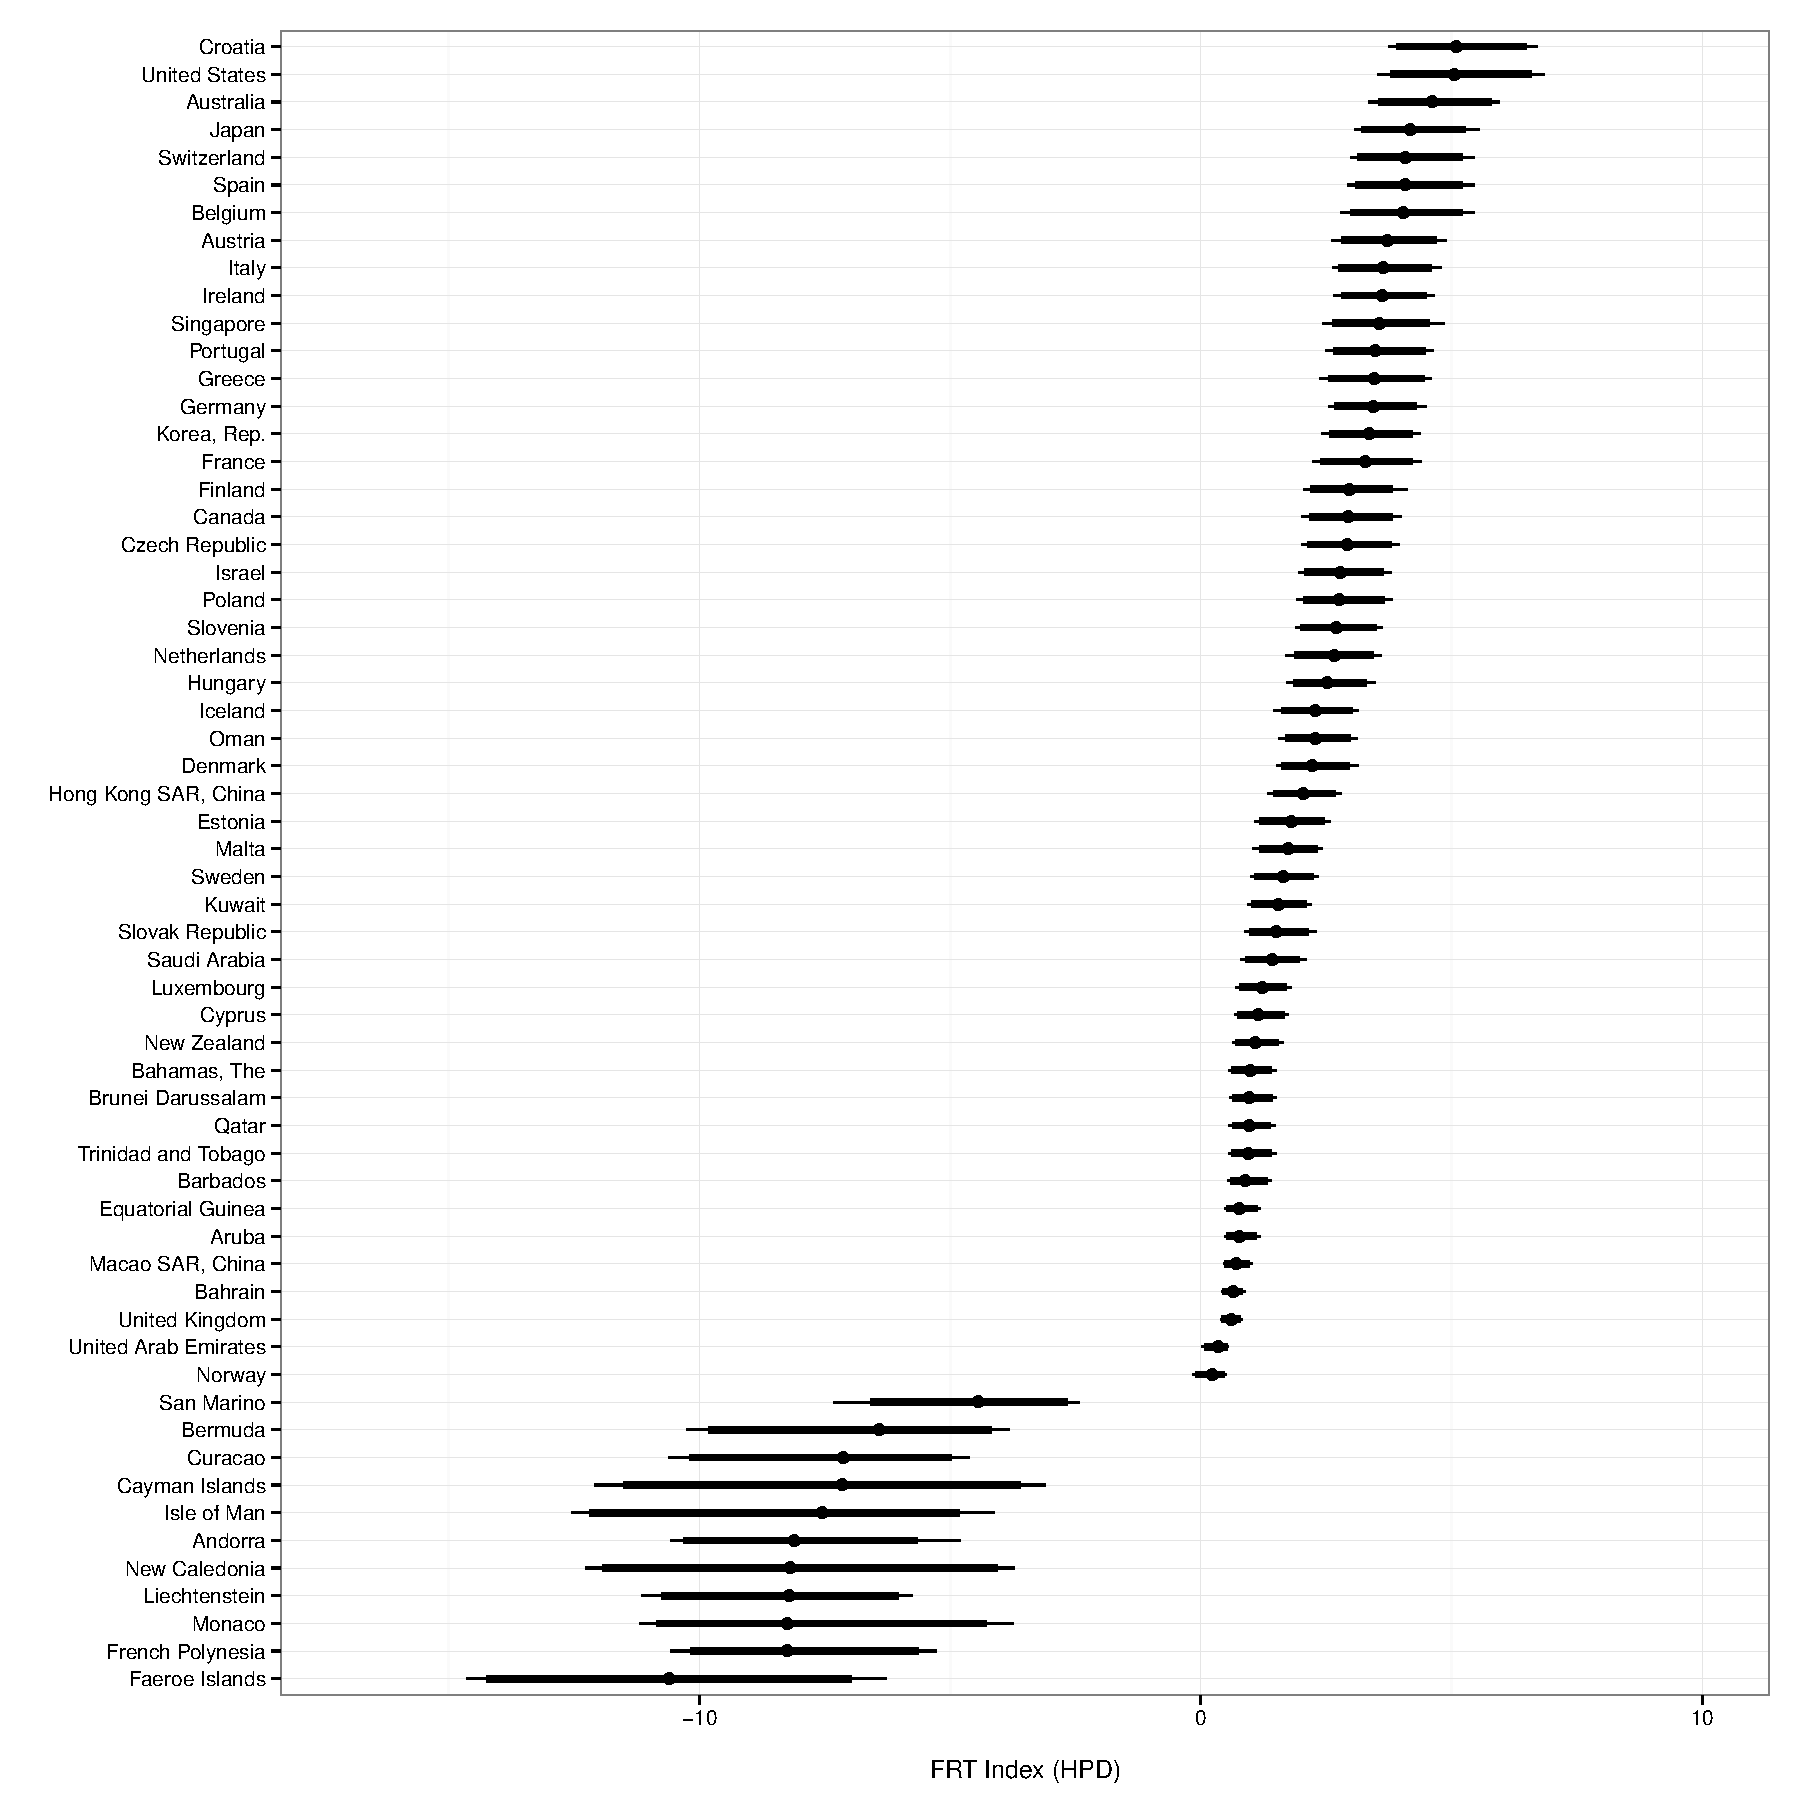
\includegraphics[scale=0.45]{figures/FRT_2007}
    \end{center}
    {\scriptsize{Thin lines represent the 95\% highest posterior density interval. Thick lines represent the 90\%.}}
\end{figure}

\begin{figure}
    \caption{Financial Regulatory Transparency Index in 2011}
    \label{FRT_2011}
    \begin{center}
        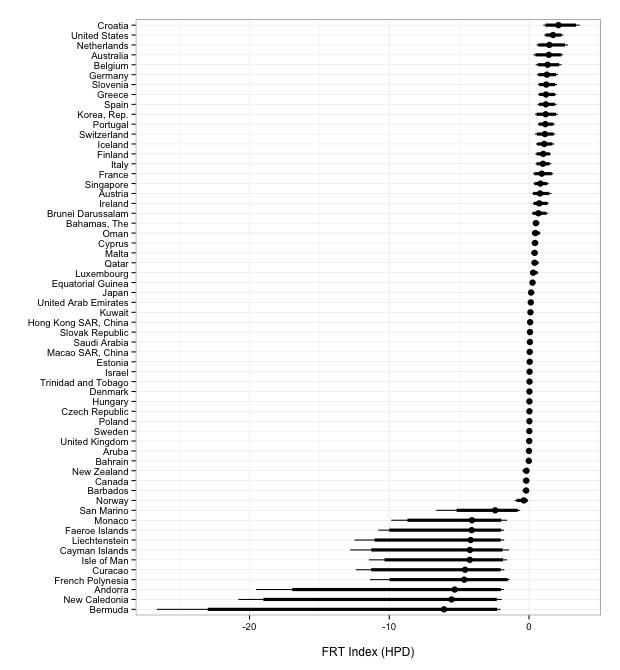
\includegraphics[scale=0.45]{figures/FRT_2011}
    \end{center}
    {\scriptsize{Thin lines represent the 95\% highest posterior density interval. Thick lines represent the 90\%.}}
\end{figure}

It's important to also note that the FRT Index provides distinct information from more general transparency indices, such as Hollyer et al.'s HRV Index and Freedom House  

\todo{COMPARE COUNTRY PLACEMENT TO HRV INDEX, ESPECIALLY SWEDEN.}

\begin{figure}
    \caption{Financial Regulatory Transparency Index for Hungary}
    \label{FRTHungary}
    \begin{center}
        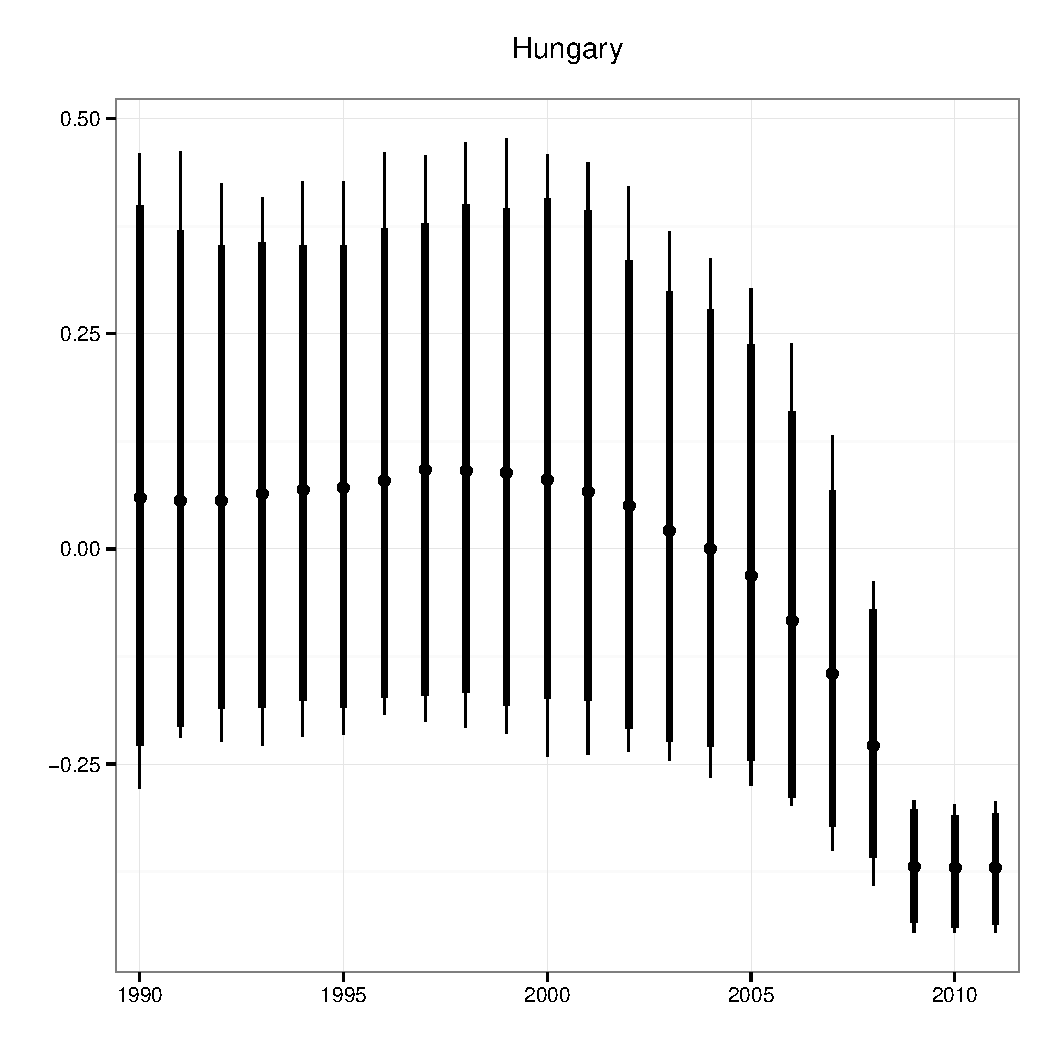
\includegraphics[scale=0.5]{figures/FRT_Hungary}
    \end{center}
\end{figure}

\subsection{Indicator difficulty}

\subsection{Indicator discrimination}


[OTHER TRANSPARENCY INDICATORS TO COMPARE AGAINST?]

\section{Preliminary Associations}

To demonstrate the potential usefulness of the FRT Index we examine a number of associations between the Index and the occurrence and potential occurrence of financial crisis.

[ASSOCIATION WITH ECONOMIC BUREAUCRATIC CAPACITY]
[Z-SCORE (PROB. OF BANK DEFAULT) AS DEPENDENT VARIABLE]

\section*{Conclusion}

\bibliographystyle{apsr}
\bibliography{FRTIndex}

\section*{Supplementary Materials}

\todo[inline]{TRACE PLOTS AND OTHER DIAGNOSTICS}


\end{document}